\section{Optimal Experimental Design Considerations}

In this section we return to the nonlinear examples presented in the previous chapter and address some choices made in how the experiment was performed.
By revisiting the examples, we demonstrate that the decisions made regarding measurement equipment and/or location have an impact on the reduction of uncertainty and accuracy of the MUD point.
Furthermore, we want to show that the choices made in the experimental design of previous examples were made for reasons of convenience of exposition.
Changing these assumptions does not later the viability of the MUD point as an alternative estimator for use parameter identification problems.

We study the impact of more precise measurement devices on the convergence rates for the parameter estimates.
First we return the problem of estimating the rate of exponential decay by incorporating measurements taken in time into the WME map from [TK - ch4 section here].
To complement these results, we show them alongside ones generated with equipment that measures at twice the temporal frequency.

Next, we study the same question of the impact of measurement precision for the PDE problem introduced in \ref{subsec:pde-example}.
A similar complementary problem is solved where information about the sensitivity of measurement locations is used to inform improved placement of a hundred sensors.
In this example, we walk through the sorts of analyses a modeler might conduct in order to select an experimental design through simulation and show a significant improvement in the accuracy of the MUD point.


%%%%%%%%%%%%%%%%%%%%%%%%%%%%%%%%%%%%%%%%%%%%%%%%%%%%%%%%%%%%%%%%%%%%
%%%%%%%%%%%%%%%%%%%%%%%%%%%%%%%%%%%%%%%%%%%%%%%%%%%%%%%%%%%%%%%%%%%%
\subsection{ODE Example Revisited}
One way by which modelers can improve the quality of parameter estimates is by collecting more data.
We consider what would happen if our measurement equipment were able to capture twice as many observations.

%%%%%%%%%%%%%%%%%%%%%%%%%%%%%%%%%%%%%%%%%%%%%%%%%%%%%%%%%%%%%%%%%%%%
\subsubsection{Different Measurement Equipment}
Instead of using equipment that operates at $100$Hz, we take $200$ measurements every second, resulting in 400 equispaced observations for $t \in (1,3)$.
All other choices involved in the experiment (assumed equipment tolerance, number of trials, parameter samples), are kept the same.
We refer to this setup wit faster measurement equipment as the ``alternative'' design.


We show the resulting predictions for the signal using MUD points from twenty repeated trials in Figure~\ref{fig:ode-alt-reference} using the first twenty (middle) and all of the measurements (bottom).
The top of the figure shows the solution from the original setup \ref{fig:ode-reference} for visual comparison.
The true signal is well-recovered even with a small subset of the data collected.
By the time all measurements are used, the stability of the solutions\---with respect to the noise that may have polluted them\---is evidenced by the fact that the red lines representing solutions disappear against the backdrop of the true signal in black.

\begin{figure}[htbp]
  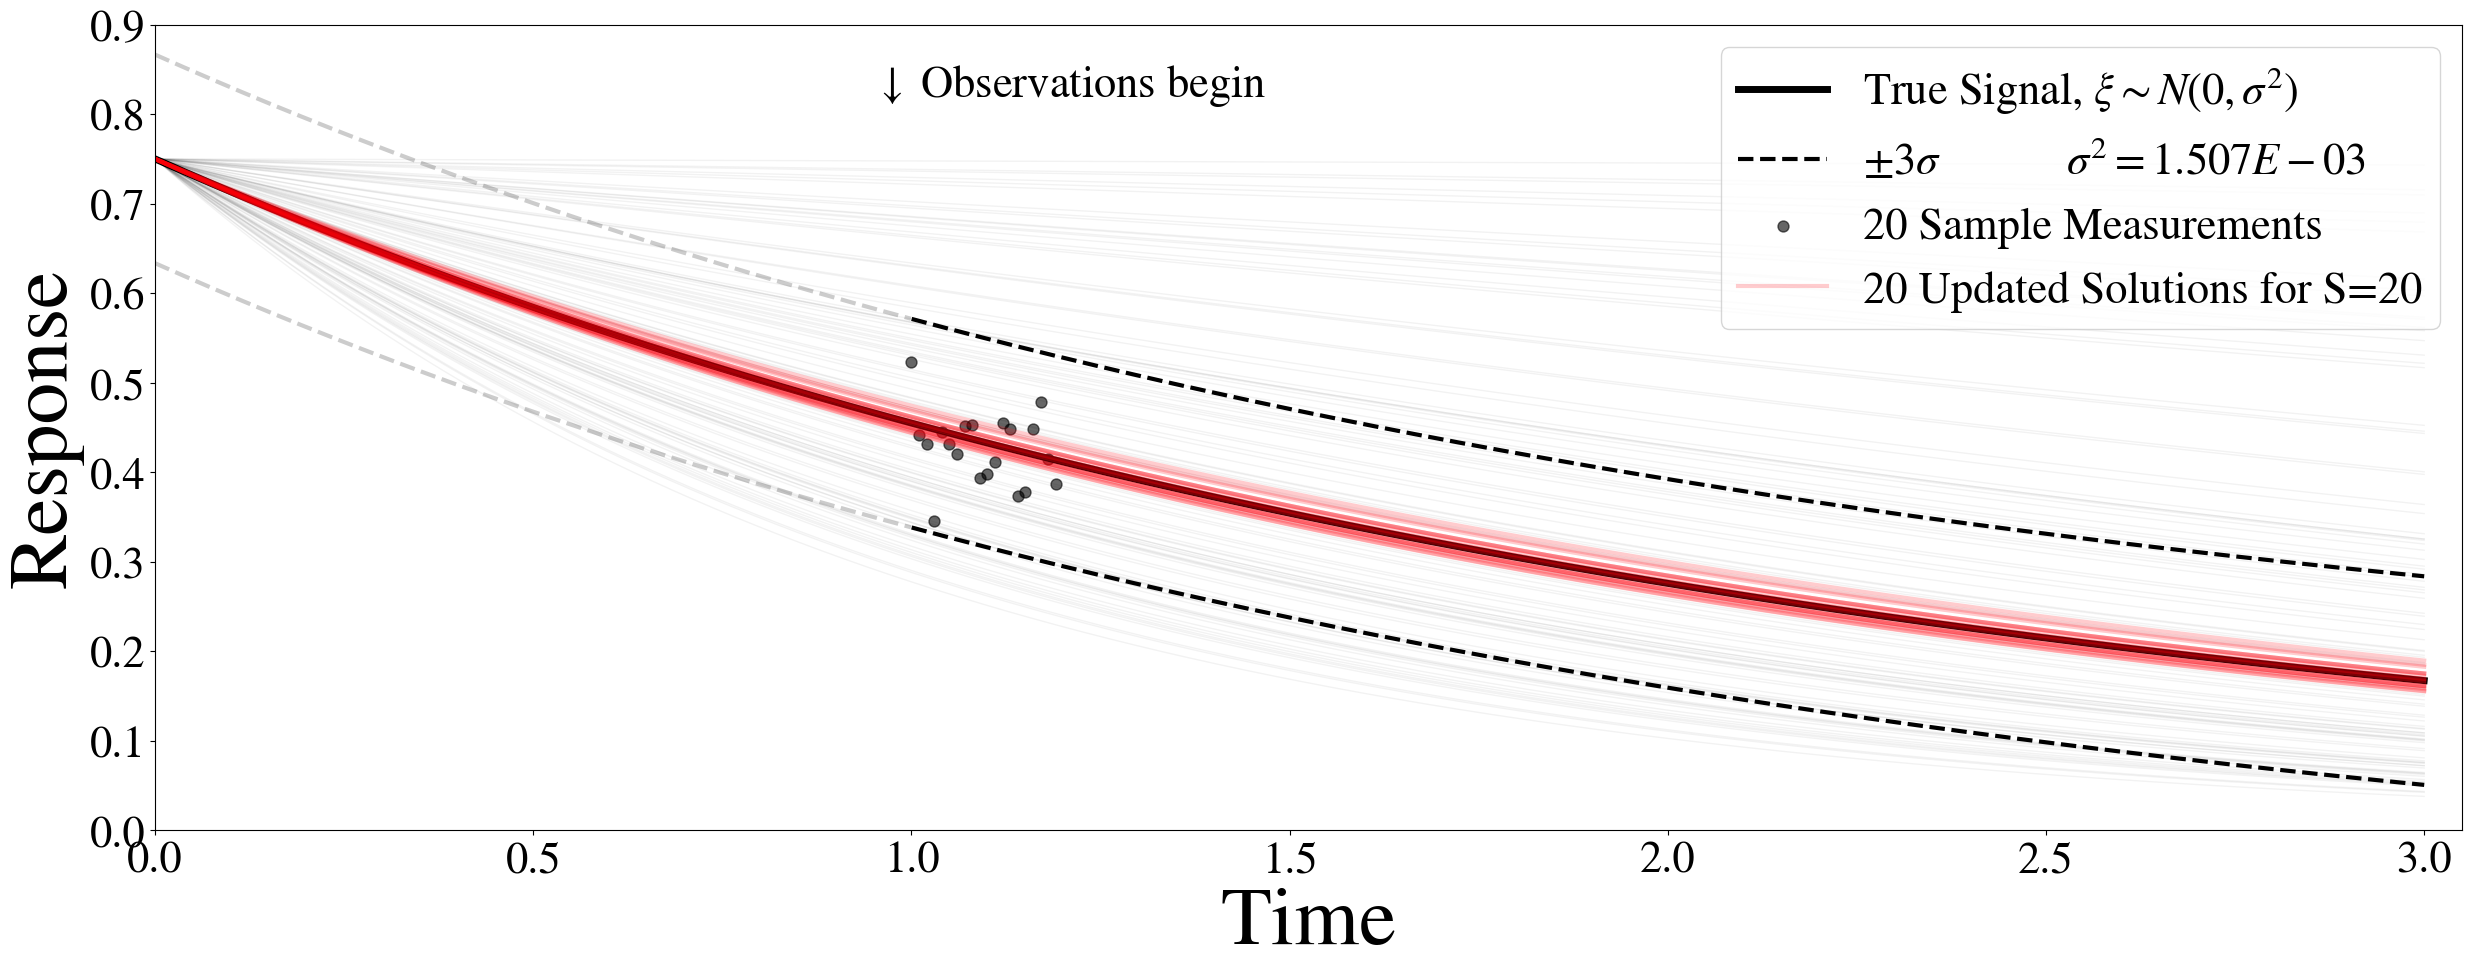
\includegraphics[width=\linewidth]{figures/ode/ode_20_reference_solution}
  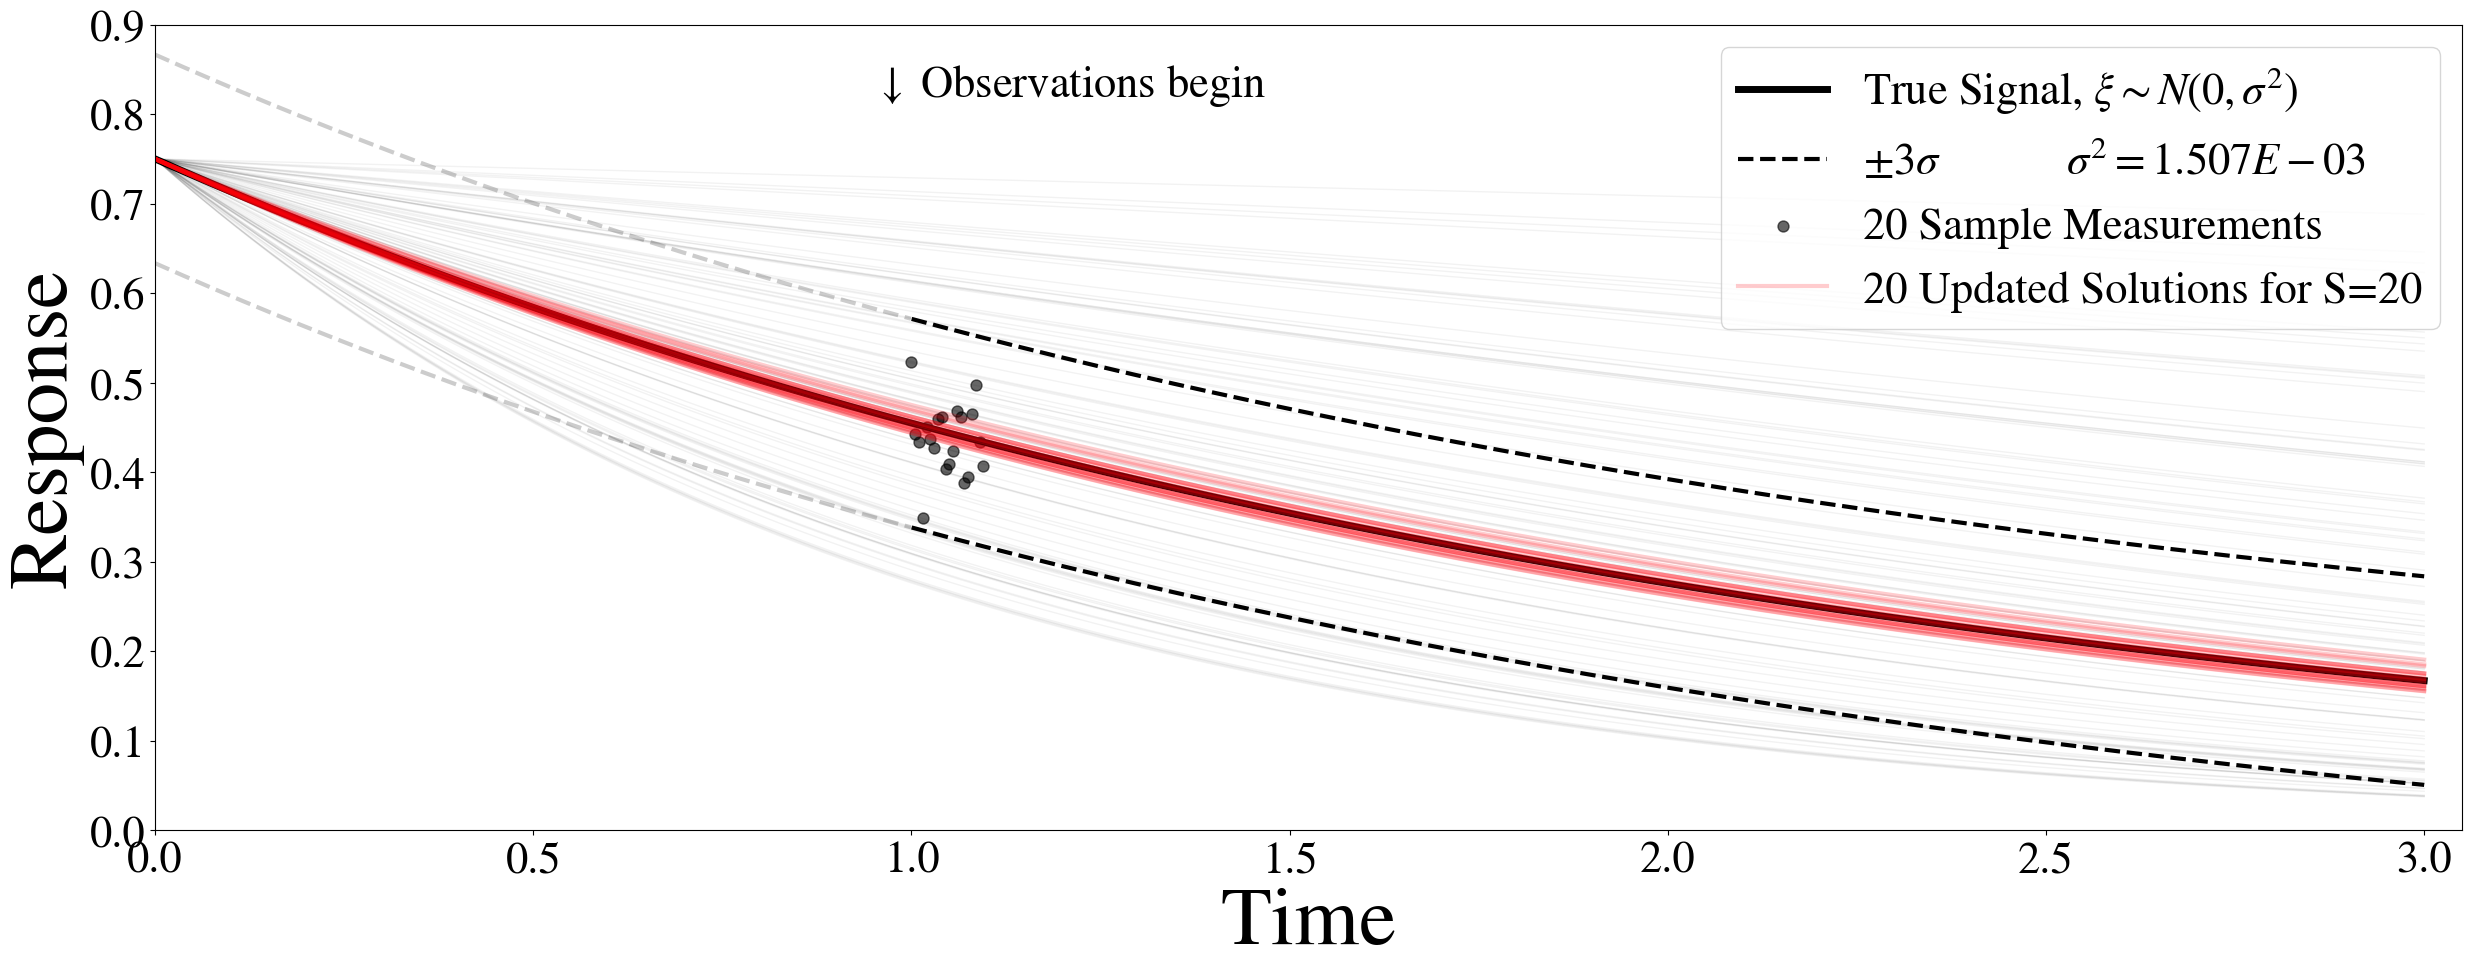
\includegraphics[width=\linewidth]{figures/ode/ode-alt_20_reference_solution}
  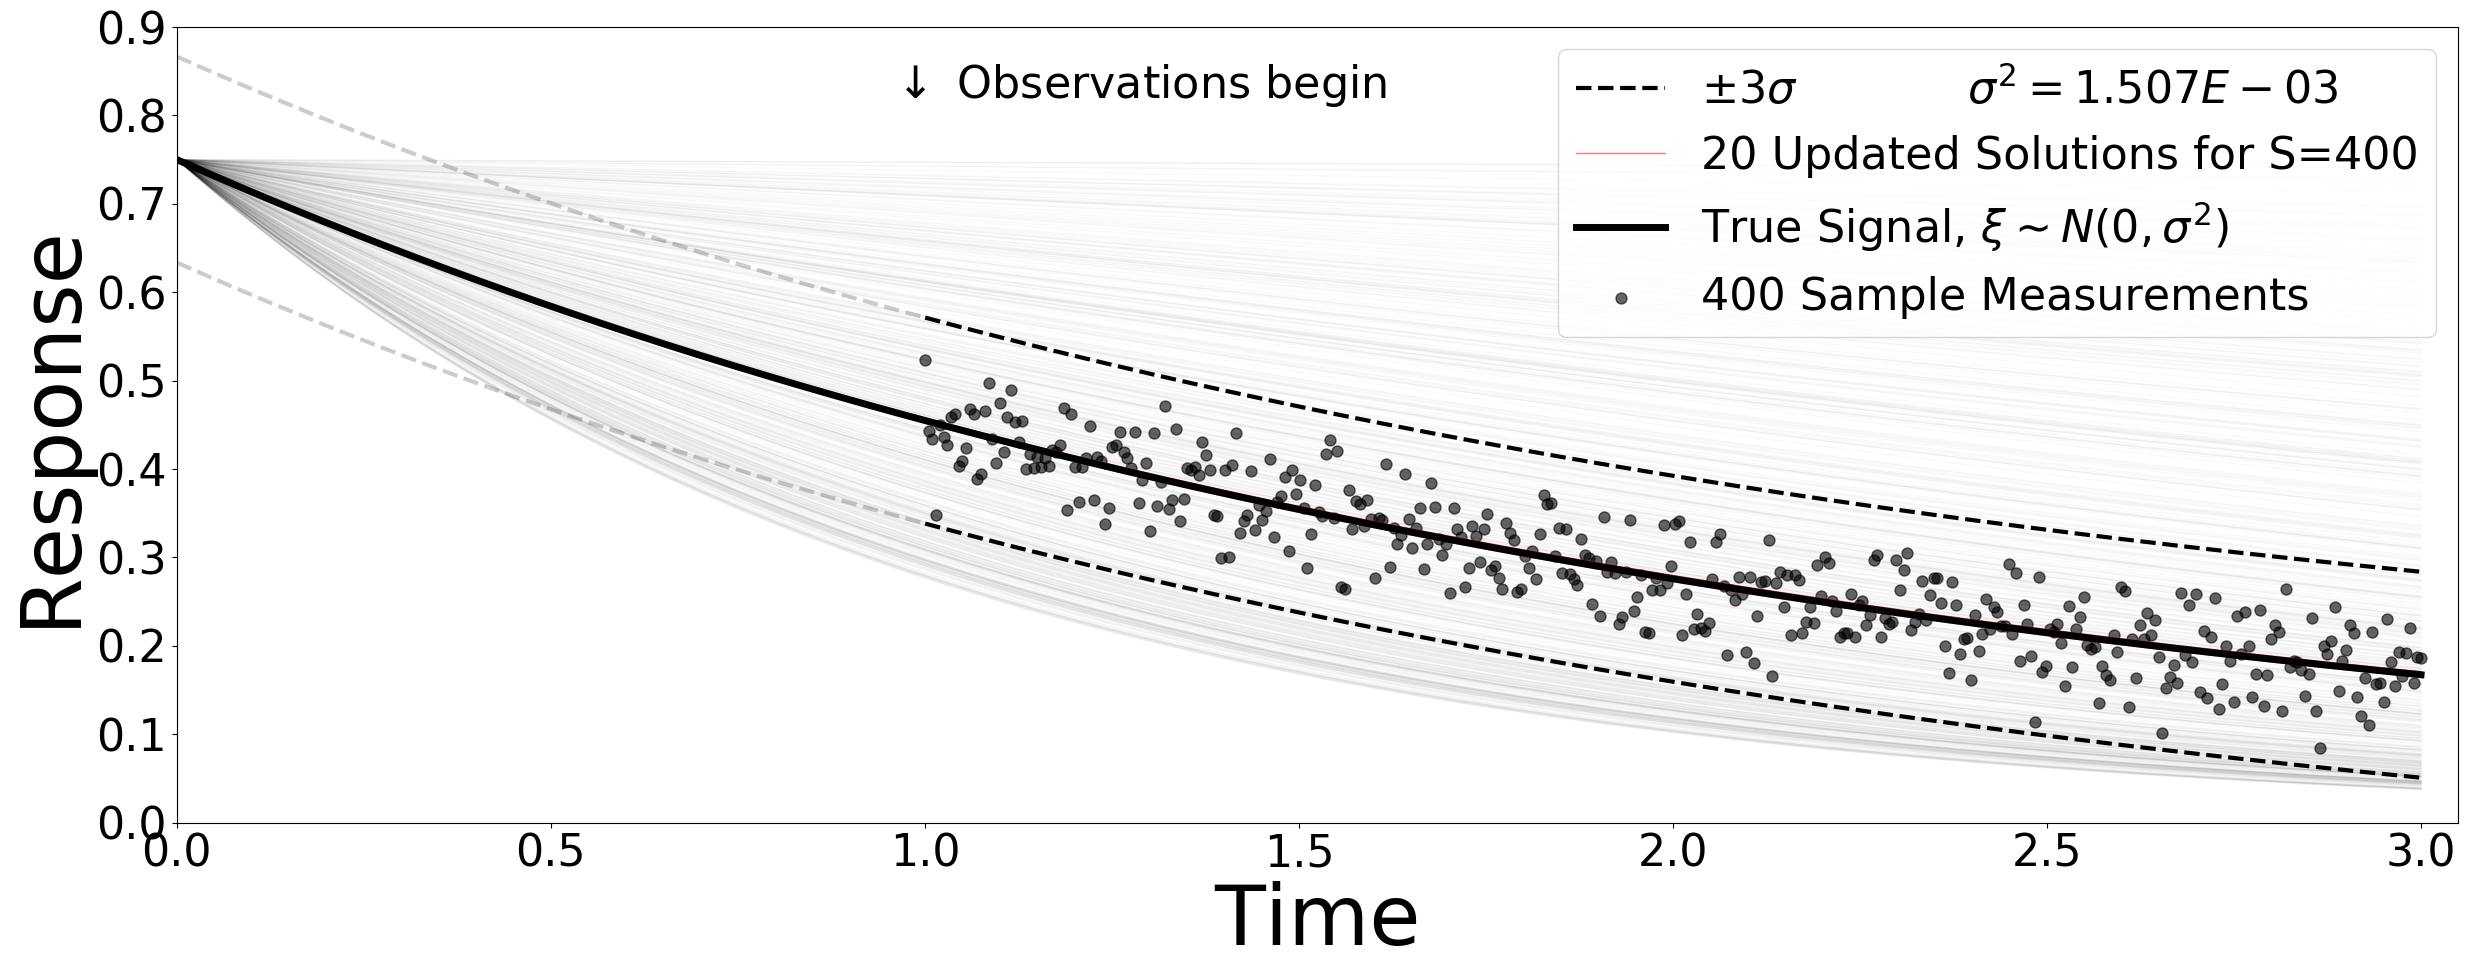
\includegraphics[width=\linewidth]{figures/ode/ode-alt_400_reference_solution}
  \caption{Gray lines are the initial parameter samples.
  The true signal (black) is well-recovered by the MUD estimates (red).
  (Top): First twenty measurements used to solve the original problem.
  (Middle): First twenty measurements used to solve the alternative problem.
  (Bottom): The entire value $\param_i$ ($1\leq i \leq N$), in the sampled parameter set.
  }
  \label{fig:ode-alt-reference}
\end{figure}

To quantify accuracy and stability of the MUD solutions, we solve the problem for the same choices of $S$ as the original problem (with the addition of $S=400$).
We show the resulting error plots for convergence in the right half of Figures~\ref{fig:ode-convergence-obs}, juxtaposed against the original experimental design with $100$Hz equipment.

\begin{figure}[htbp]
  \centering
  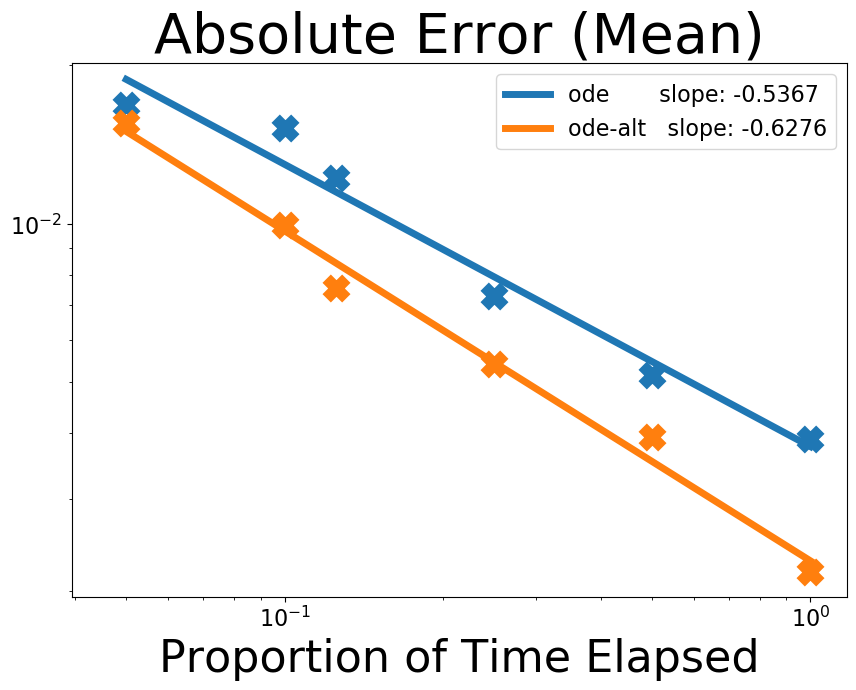
\includegraphics[width=0.475\linewidth]{figures/ode/ode_convergence_mud_obs_mean}
  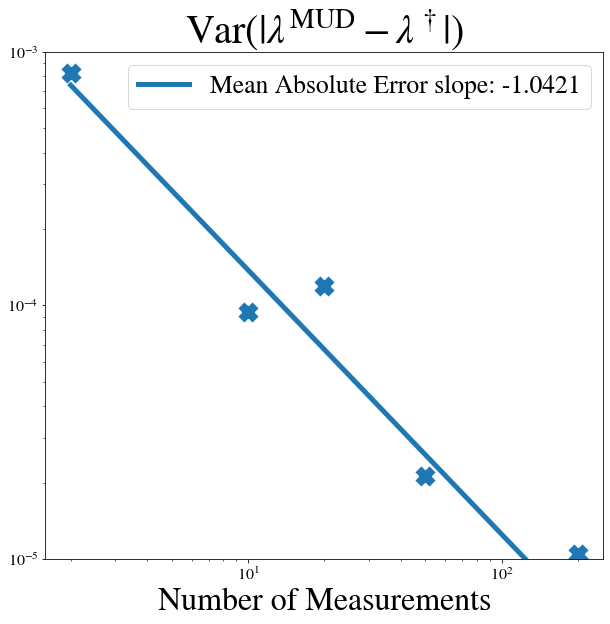
\includegraphics[width=0.425\linewidth]{figures/ode/ode_convergence_mud_obs_var}

  \caption{Convergence of the MUD point given $N=1E3$ model evaluations for increasing numbers of observations for randomly placed sensors.
  Convergence rates are estimated using first-order linear regressions in $\text{log}_{10}$-space.
  $100$Hz equipment demonstrates a reduction of uncertainty and improvement in precision as $S$ increases towards $200$.
  We observe the same rates of convergence for the alternative equipment and note the (slightly) lower overall error for equal numbers of measurements ($S=200$ corresponding to $t\in (1,2)$ in this formulation).
  }
  \label{fig:ode-convergence-obs}
\end{figure}

The convergence rates are similar (shown in the legend of \ref{fig:ode-convergence-obs}), and reduction in uncertainty is almost negligible at a given $S$.
However, we note that in the alternative setup, for an equal number of measurements, the time elapsed is half of that in the original due to the different equipment being used.
To this end, we estimate convergence rates with respect to the time elapsed in the experiment rather than number of measurements used, and notice that the alternative setup (orange) exhibits much lower error at a given point of time.
This implies that we can achieve similar results with a shorter observational window by using equipment that allows for faster observations.



%%%%%%%%%%%%%%%%%%%%%%%%%%%%%%%%%%%%%%%%%%%%%%%%%%%%%%%%%%%%%%%%%%%%
\FloatBarrier
%%%%%%%%%%%%%%%%%%%%%%%%%%%%%%%%%%%%%%%%%%%%%%%%%%%%%%%%%%%%%%%%%%%%

\subsubsection{Impact of Equipment Precision}
To achieve higher precision in the estimate of the MUD point, one can use more precise measurement equipment.
We expect that a method designed to address parameter estimation would see an improvement in accuracy  if the data is collected with more precise instruments.
Here we show that this is indeed the case for the time-series example introduced earlier by considering choices of $\tau = 0.1, 0.05, 0.01, \text{ and } 0.005$ for $\mathbb{P}( \abs{\xi} < \tau ) = 99\%$ to select our $\sigma$ in our normal additive noise model.
We sequentially incorporate $S=5, 10, 15, 20, 25, 50, 100, \text{ and } 200$ measurements and study the error in our estimate of $\paramref$.



\begin{figure}[htbp]
  \centering
  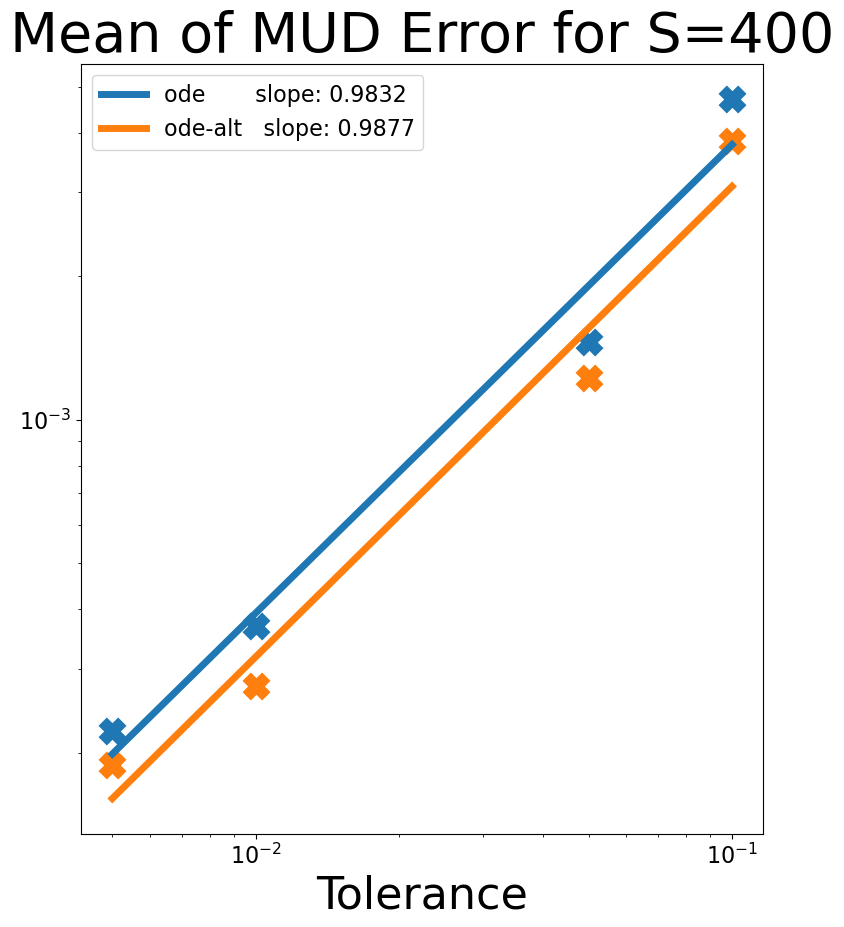
\includegraphics[width=0.475\linewidth]{figures/ode/ode_convergence_mud_std_mean}
  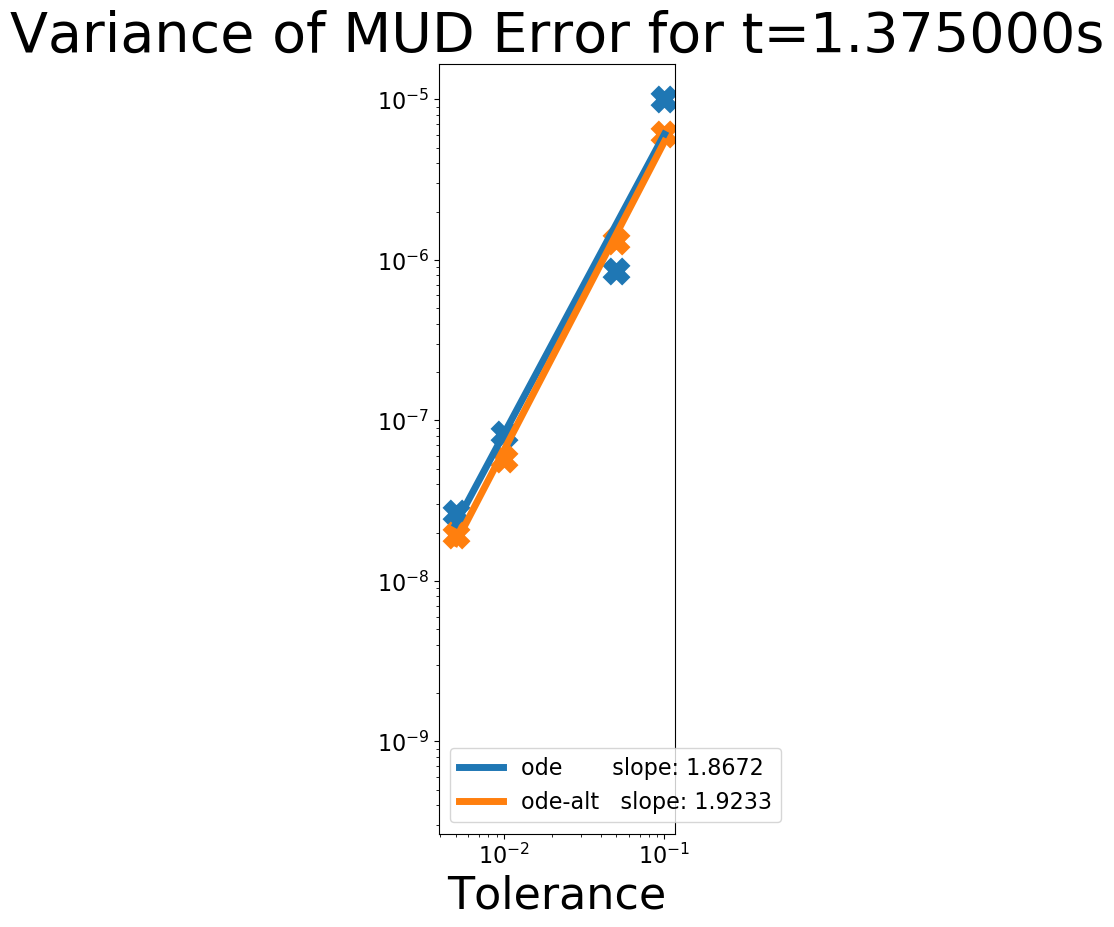
\includegraphics[width=0.425\linewidth]{figures/ode/ode_convergence_mud_std_var}

  \caption{Convergence of the MUD point given $N=1E3$ model evaluations incorporating measurements at a fixed point in time.
  As more precise measurements are incorporated, the accuracy and precision of the MUD solution improves.
  }
  \label{fig:ode-convergence-std}
\end{figure}

In Figure~\ref{fig:ode-convergence-std}, we study the absolute error's mean and variance as our measurement equipment gets more precise (lower tolerance), for both the $100$Hz (ode) and $200$Hz (ode-alt) variants of sensors we are simulating.
In the left half of the figure, we find that the convergence rates for the two designs are nearly identical but the equipment which records twice as many measurements has a persistent reduction in error.
The right half shows the convergence in variance of the absolute error, and the vertical displacement between the two designs is visually difficult to distinguish.
However, as evidenced in the legend annotations of Fig~\ref{fig:ode-convergence-std}, the alternative design (faster equipment) exhibits an increase in the rate of convergence from 1.87 to 1.92.

We have shown that the Data--Consistent approach to solving parameter identification problems manages to generalize to problems involving time-series data from a single Quantity of Interest.
We now turn our attention to an example where instead of temporal measurements, we incorporate spatial data to solve another 1-D parameter identification problem.

%%%%%%%%%%%%%%%%%%%%%%%%%%%%%%%%%%%%%%%%%%%%%%%%%%%%%%%%%%%%%%%%%%%%
%%%%%%%%%%%%%%%%%%%%%%%%%%%%%%%%%%%%%%%%%%%%%%%%%%%%%%%%%%%%%%%%%%%%
\FloatBarrier
%%%%%%%%%%%%%%%%%%%%%%%%%%%%%%%%%%%%%%%%%%%%%%%%%%%%%%%%%%%%%%%%%%%%
%%%%%%%%%%%%%%%%%%%%%%%%%%%%%%%%%%%%%%%%%%%%%%%%%%%%%%%%%%%%%%%%%%%%
\subsection{Elliptic PDE Example}\label{sec:pde-example}
We make a slight modification to the Poisson problem from \ref{subsec:nonlinear-example} to make it into a one-dimensional parameter identification problem.
We briefly summarize the experimental set-up again for convenience of the reader.
Consider the following Poisson problem defined on a unit domain $\Omega$:
\begin{equation}\label{eq:pde-equation}
\begin{cases}
\hfill -\nabla \cdot \nabla u &= f \quad\text{on } \Omega \\
\hfill u &= 0 \quad\text{ on } \Gamma_T \cup \Gamma_B \\
\hfill \frac{\partial u}{\partial \mathbf{n}} &= g(x,\param) \quad\text{ on } \Gamma_L \\
\hfill \frac{\partial u}{\partial \mathbf{n}} &= 0 \quad\text{ on } \Gamma_R
\end{cases}
\end{equation}
where $(x_1, x_2) \in \Omega = (0,1)^2$, $\Gamma_T$ is the top, $\Gamma_B$ is the bottom, $\Gamma_L$ and $\Gamma_R$ left and right, respectively.
$\frac{\partial u}{\partial \mathbf{n}}$ denotes the outward normal direction.
We select $g=\param \sin(\pi x_2)$, and show the response surface for our given choice of $\param = 3$ in the left of Figure~\ref{fig:pde-response}, with darker colors representing more negative values.
Our initial density is chosen to be uniform over the interval $\Lambda = (1,5)$.
$f$ is chosen to be $10\exp\{-\frac{(x_1-0.5)^2 + (x_2 - 0.5)^2}{0.02}\}$


We are interested in demonstrating the impact of incorporating more measurements on our ability to estimate $\paramref$.
This poses a problem for this particular experimental design since it will heavily rely on the way in which the sensor grid is indexed.
One could place a regular grid of sensors in the interior of $\Omega$ to simulate a structured sensor array.
However, observe that the response surface shown on the left panel of Figure~\ref{fig:pde-response} exhibit vertical symmetry about the line $x_2=0.5$ (as a result of our choice of $g$).
For example, if the first half of indexed sensors corresponded to the bottom half of $\Omega$, the incorporation of the second half will be equivalent to having repeated observations.
To avoid these problems, we instead simulate the sensors as being placed randomly (drawn from uniform distributions), in the interior so that index-dependence becomes irrelevant and probability theory ensures the lack of truly redundant measurement locations.

%%%%%%%%%%%%%%%%%%%%%%%%%%%%%%%%%%%%%%%%%%%%%%%%%%%%%%%%%%%%%%%%%%%%
\FloatBarrier
%%%%%%%%%%%%%%%%%%%%%%%%%%%%%%%%%%%%%%%%%%%%%%%%%%%%%%%%%%%%%%%%%%%%
\subsubsection{Uninformed Sensor Placement}

We consider a selection of $S=1000$ measurement locations in the interior of the response surface chosen by sampling a uniform density over the set $(0.05, 0.95)^2 \subset \Omega$.
We show only the first hundred measurement locations in plots for visual clarity.
In the rightmost histogram of Figure~\ref{fig:pde-response}, we plot the data generated by each simulated sensor location, and note that many values are near zero as a result of being near boundaries or the right-side of $\Omega$.

\begin{figure}
\centering
  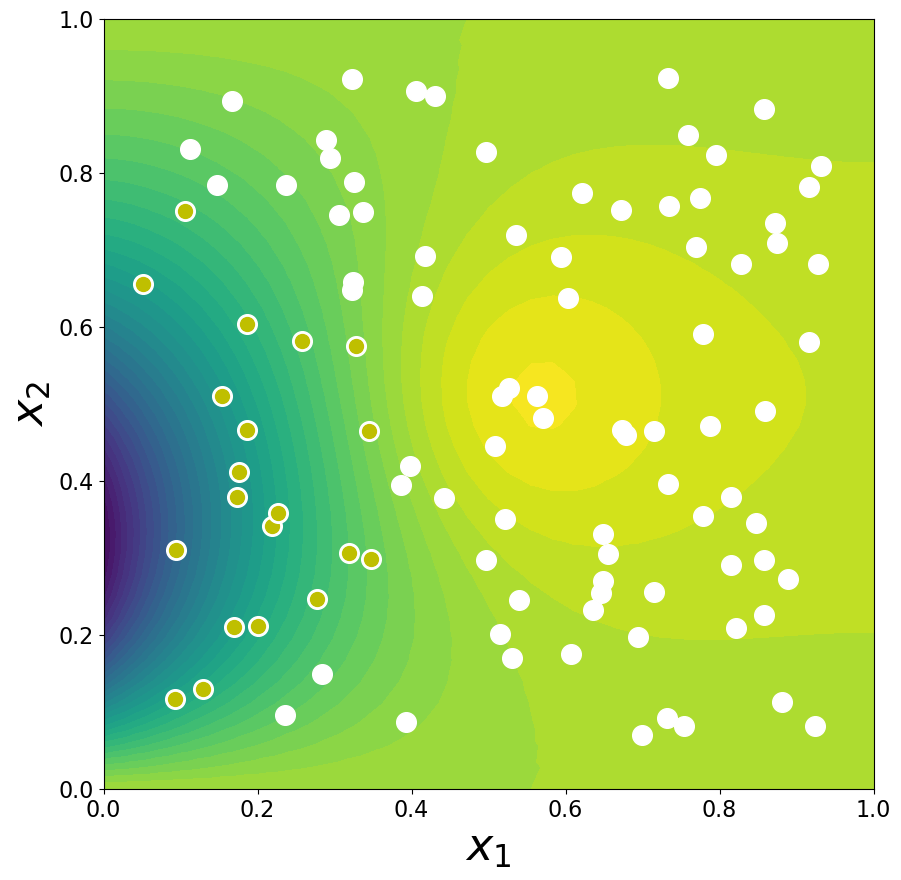
\includegraphics[width=0.35\linewidth]{figures/pde/pde_reference_solution}
  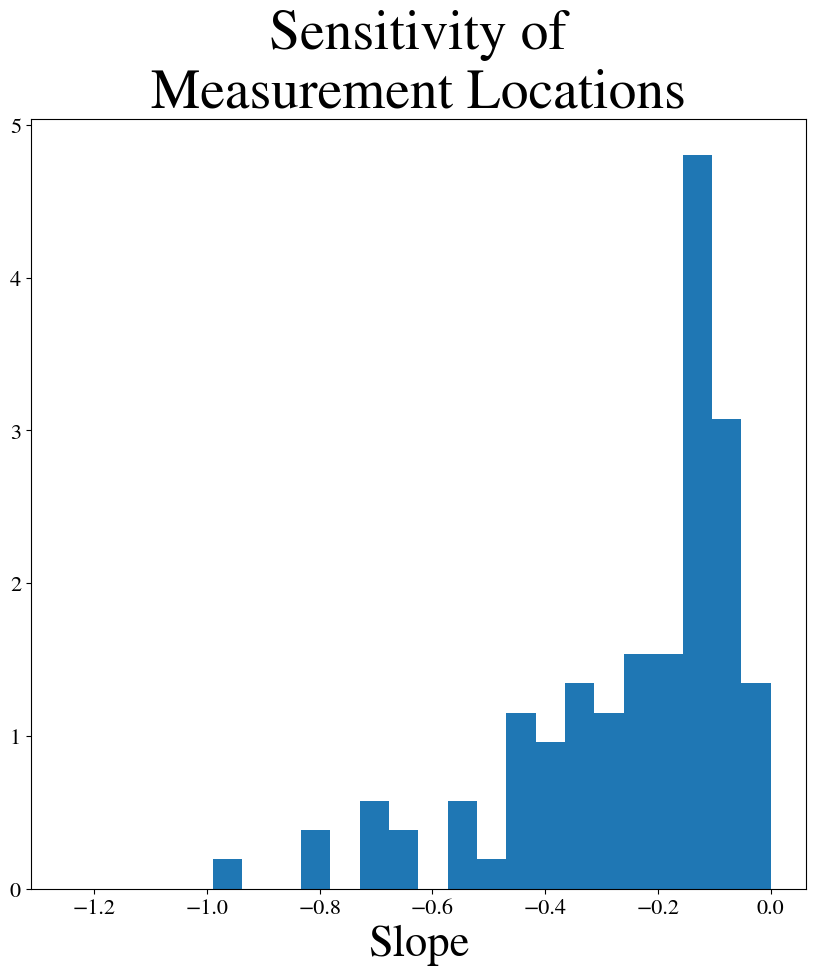
\includegraphics[width=0.35\linewidth]{figures/pde/pde_sensitivity_qoi}
  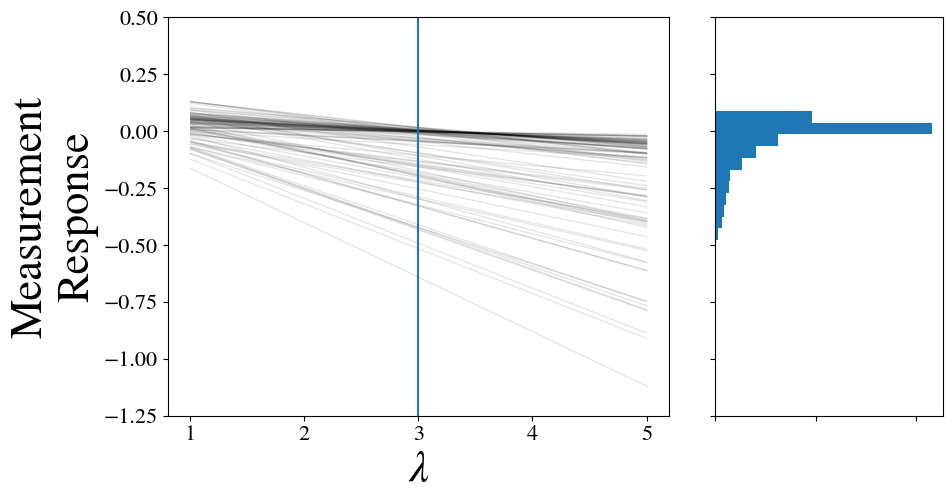
\includegraphics[width=0.675\linewidth]{figures/pde/pde_qoi_response}
\caption{(Left): The function response surface for $u$ solving \eqref{eq:pde-equation} with $S=100$ measurement locations highlighted in white.
The twenty most sensitive location markers are filled.
(Right): The derivative $\partial M_i / \partial \param$ is computed for the hundred measurement locations and the distribution of the resulting collection of slopes is plotted.
(Center): The values of the response surface at the hundred measurements is shown. The true parameter value $\paramref$ is highlighted with a vertical line, and the values of the response surface conditioned on $\paramref$ are used to form the histogram plotted vertically on the right. Many measurements are near zero.
}
\label{fig:pde-response}
\end{figure}

In the center panel of \ref{fig:pde-response}, we observe that some measurements are more sensitive than others (have steeper slopes).
The majority of measurements exhibit almost no sensitivity to changes in $\param$, visually represented by the density of nearly horizontal lines (slopes of zero).
However, some of the sensors have steep slopes, which suggests higher sensitivity to changes in $\param$.


%%%%%%%%%%%%%%%%%%%%%%%%%%%%%%%%%%%%%%%%%%%%%%%%%%%%%%%%%%%%%%%%%%%%
% \FloatBarrier
%%%%%%%%%%%%%%%%%%%%%%%%%%%%%%%%%%%%%%%%%%%%%%%%%%%%%%%%%%%%%%%%%%%%
\subsubsection{Informed Sensor Placement}
Instead of placing sensors throughout the square interior of $\Omega$ given by $(0.05, 0.95)^2$, we briefly consider how the convergence results would compare if the subdomain for sensors was better selected
In the left panel of Figure~\ref{fig:pde-response}, the most sensitive measurements are highlighted and appear near the left boundary.
Furthermore, the response surface exhibits horizontal symmetry, so we restrict locations to the bottom half of $\Omega$.
These two observations can inform a new bounding box for us to place sensors within.
We perform the same experiment for sensors placed in $(0.05, 0.25)\times(0.05, 0.5)$ (locations drawn from a uniform distribution over this region), and refer to this as the alternative experimental design.
The first hundred of the thousand sensor locations sampled is shown in the left panel of \ref{fig:pde-alt-response} and we can see that the most sensitive ones (highlighted) cluster towards the center of the left boundary, where the response surface is most negative.


\begin{figure}
\centering
  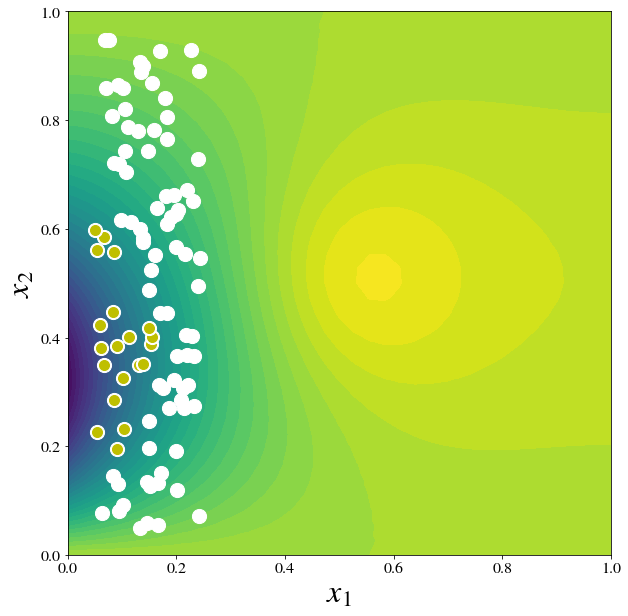
\includegraphics[width=0.35\linewidth]{figures/pde/pde-alt_reference_solution}
  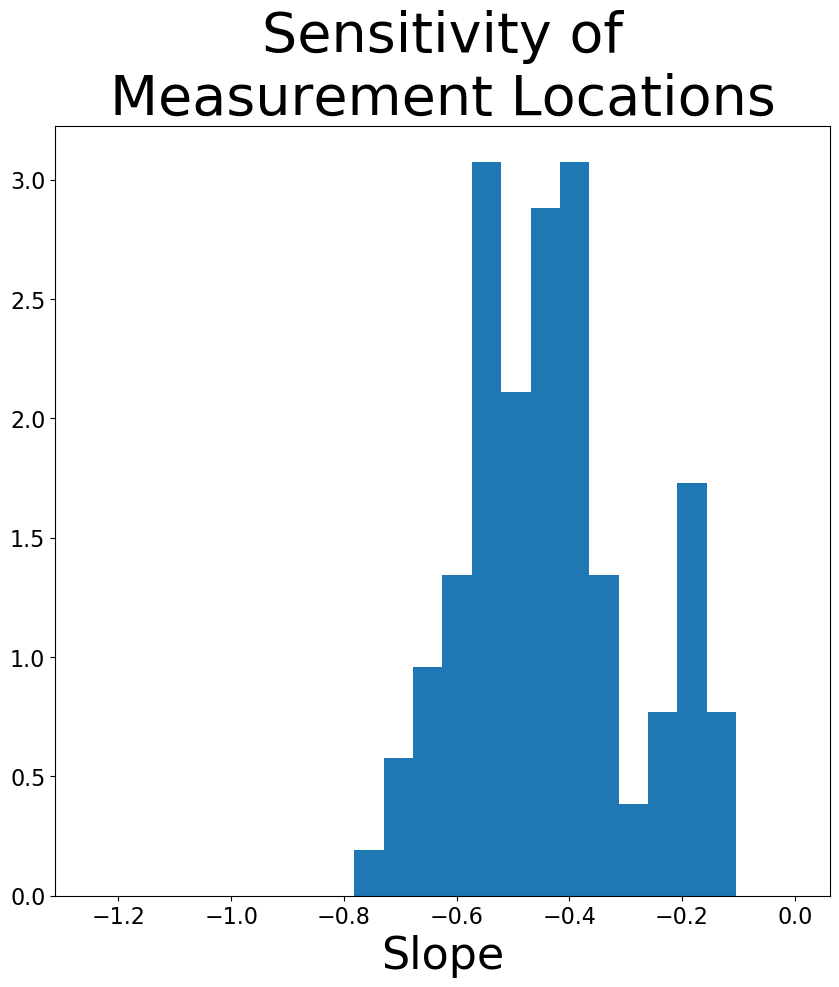
\includegraphics[width=0.35\linewidth]{figures/pde/pde-alt_sensitivity_qoi}
  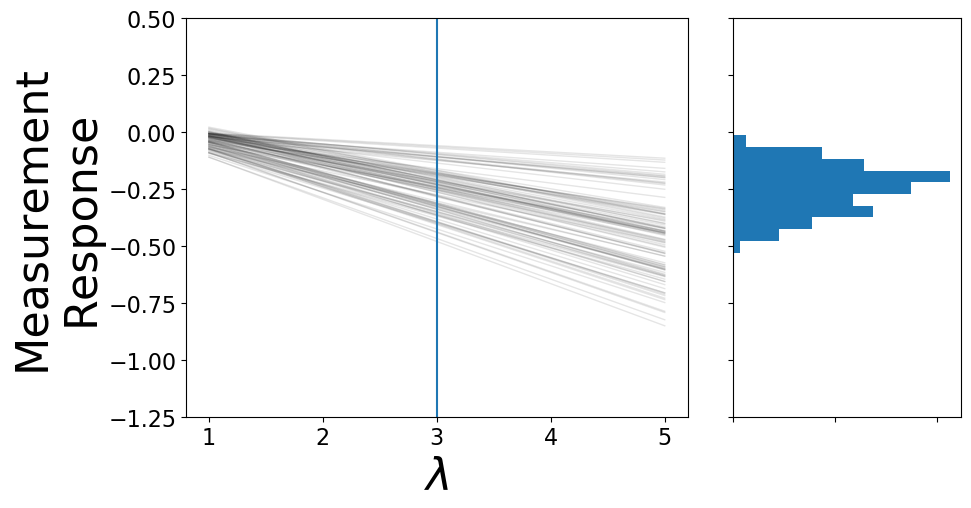
\includegraphics[width=0.675\linewidth]{figures/pde/pde-alt_qoi_response}
  \caption{The same panels as in Figure~\ref{fig:pde-response} but for the placement of sensors informed by the observations about sensitivity incorporated into the experimental design.
  The alternative placement eliminates redundancy induced by the symmetry of the response surface, and is concentrated in the regions which exhibit more sensitivity to changes in $\param$.
  As a result of these choices, we observe less measurements near zero (bottom histogram), and slopes with larger magnitude (top).
  }
\label{fig:pde-alt-response}
\end{figure}

For this alternative design, we show the sensitivity of sensors in the center of \ref{fig:pde-alt-response} and note that there are fewer sensors which exhibit low sensitivity to changes in $\paramref$ in contrast to \ref{fig:pde-response}.
The slopes are again shown in the center of the figure and exhibit a bimodal distribution with a larger portion of the measurements having slopes with magnitude 4-6 times greater than the mode in the center of \ref{fig:pde-response}.
There are also less measurements which take values near zero as well, shown in the rightmost panel of the figures.
Whereas the original design had an strong decay in its distribution of measurement values, the alternative shows a much more symmetric distribution.


%%%%%%%%%%%%%%%%%%%%%%%%%%%%%%%%%%%%%%%%%%%%%%%%%%%%%%%%%%%%%%%%%%%%
\FloatBarrier
%%%%%%%%%%%%%%%%%%%%%%%%%%%%%%%%%%%%%%%%%%%%%%%%%%%%%%%%%%%%%%%%%%%%
\subsubsection{Comparison of SIP Solutions with Different QoI Maps} 

We are interested in knowing how the uncertainty around the parameter estimate (the MUD point) changes as we incorporate more (noisy) data.
To generate convergence plots, we solve the problem repeatedly for $S = 5, 10, 15, 20, 25, 50, 100, 250, 500, \text{ and } 1000$ and take the mean and variance of the twenty trials for each value of $S$.
Consider the convergence plots in Figure~\ref{fig:pde-convergence-obs}, which demonstrates the impact of increasing $S$ on our ability to resolve $\paramref$.

\begin{figure}
  \centering
  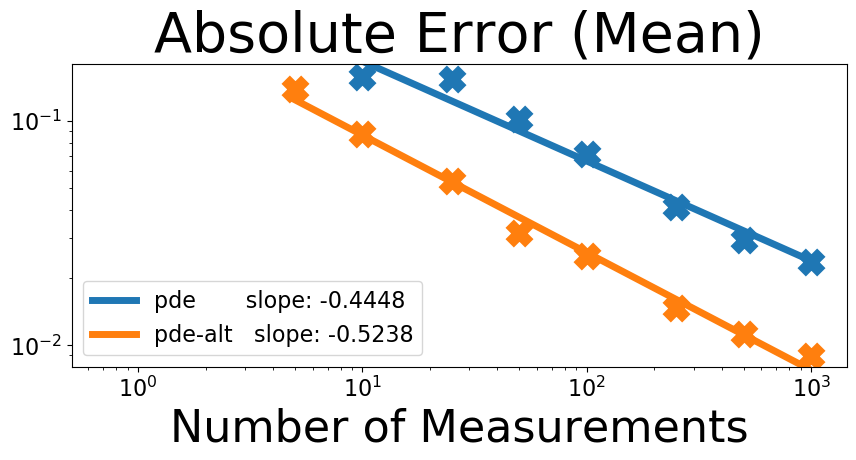
\includegraphics[width=0.475\linewidth]{figures/pde/pde_convergence_mud_obs_mean}
  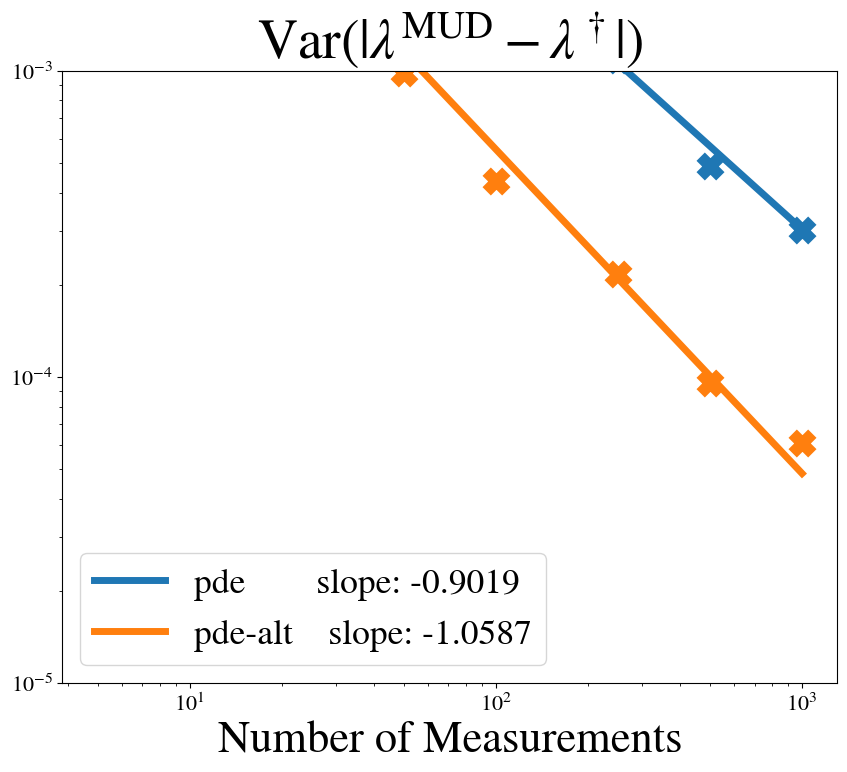
\includegraphics[width=0.475\linewidth]{figures/pde/pde_convergence_mud_obs_var}
  \caption{Convergence of the MUD point (given $N=1E3$ model evaluations) for increasing numbers of observations for randomly placed sensors.
  We observe similar rates of convergence for both arrangements of measurement locations, with a marked improvement in both accuracy and precision when an informed placement is used.
  }
  \label{fig:pde-convergence-obs}
\end{figure}

It appears in the right half of Figure~\ref{fig:pde-convergence-obs}, that two decimal places of accuracy can be achieved with approximately $250$ samples instead of the $1000$ required in the left-half.


Similar to \ref{fig:ode-convergence-std}, we demonstrate that using more sensitive measurement equipment improves the estimation of the MUD point by considering the same choices for $\tau$, the precision of the sensors.
In Figure~\ref{fig:pde-convergence-std}, we study the impact of more precise measurement equipment on the absolute error's mean and variance.


\begin{figure}[htbp]
  \centering
  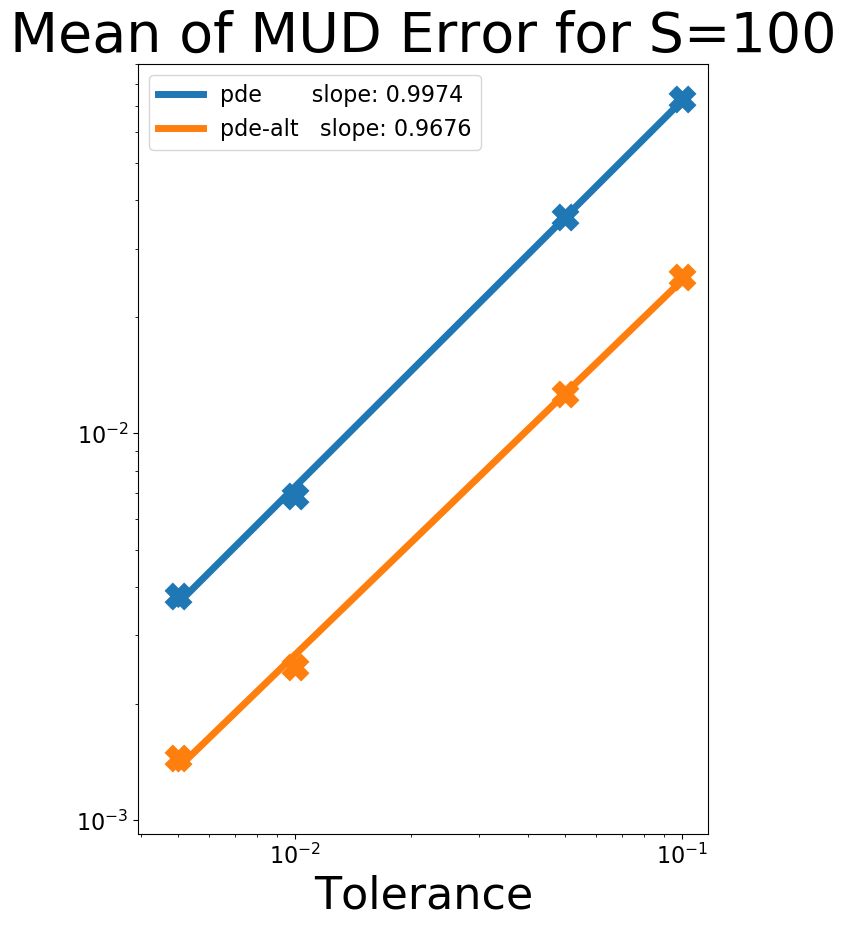
\includegraphics[width=0.475\linewidth]{figures/pde/pde_convergence_mud_std_mean}
  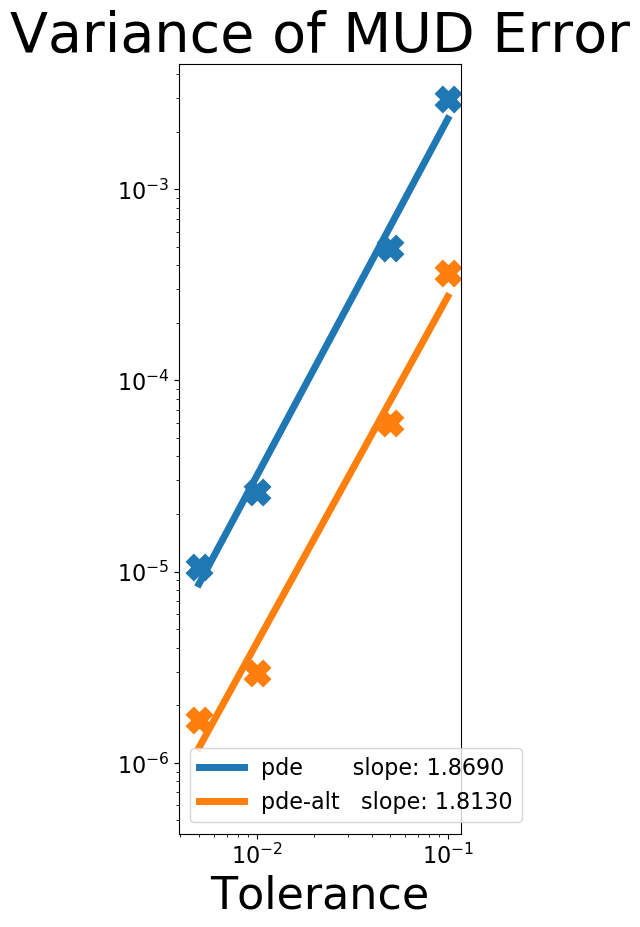
\includegraphics[width=0.475\linewidth]{figures/pde/pde_convergence_mud_std_var}
  \caption{Convergence of the MUD point given $N=1E4$ model evaluations for different measurement precision for randomly placed sensors, incorporating $S=100$ measurements.
  We note that the convergence rates are the same but the overall accuracy and precision improve when sensors are placed in regions of $u$ that exhibit higher sensitivity to changes in $\param$.
  }
  \label{fig:pde-convergence-std}
\end{figure}


The convergence results for the original experimental design demonstrate that even randomly placed sensors in the interior of $\Omega$ are suitable for parameter estimation.
However, when we considered sensors that were placed with considerations of knowing the family of curves to which $g$ belonged, we were able to extract much more information from our measurement equipment by placing sensors in different locations.
Using our alternative experimental design, we saw a reduction of uncertainty that was tangible in both Figures~ \ref{fig:pde-convergence-obs} and \ref{fig:pde-convergence-std}, represented by the persistent vertical displacement between the regression lines for convergence.


%%%%%%%%%%%%%%%%%%%%%%%%%%%%%%%%%%%%%%%%%%%%%%%%%%%%%%%%%%%%%%%%%%%%
%%%%%%%%%%%%%%%%%%%%%%%%%%%%%%%%%%%%%%%%%%%%%%%%%%%%%%%%%%%%%%%%%%%%
\FloatBarrier
%%%%%%%%%%%%%%%%%%%%%%%%%%%%%%%%%%%%%%%%%%%%%%%%%%%%%%%%%%%%%%%%%%%%
%%%%%%%%%%%%%%%%%%%%%%%%%%%%%%%%%%%%%%%%%%%%%%%%%%%%%%%%%%%%%%%%%%%%
\subsection{Concluding Remarks for Examples}

These examples demonstrate that Data--Consistent Inversion can be used for parameter identification as a viable alternative to existing methods.
The problems in this section have involved one-dimensional output spaces, and solely demonstrate one method by which measurements can be transformed into a QoI map.
The problems have also involved one-dimensional parameter spaces, limiting the useful dimension of the QoI map we construct.
We address these concerns in the next section by extending the previous (PDE) example to a vector-valued analogue with the original experimental design for collecting measurements in $(0.05, 0.95)^2$.

We point out that incorporating available observations as we have done in the previous two examples leaves the output space scalar-valued.
As the number of parameters grows, this output dimension resulting from such an approach effectively stays fixed.
These situations are particularly when the DCI approach becomes advantageous over other methods, as it is less sensitive to mistakes in modeling assumptions than other methods for solving inverse problems as we saw with the linear examples in ch4 [TK - refer back to section 4 and 6].
One can incorporate a much wider variety of prior beliefs about the relative likelihoods of parameters before data is collected without compromising predictive error.
The DCI approach guarantees that the functional defined (for us, the weighted mean error) will remain accurate in spite of any encoded assumptions that are somehow at odds with data that is subsequently collected.
